\documentclass{scrartcl}
\usepackage[a4paper,left=0mm,top=0mm,right=0mm,bottom=0mm,footskip=0in]{geometry}
\usepackage{tikz}
\usepgflibrary{patterns}
\begin{document}
\thispagestyle{empty}
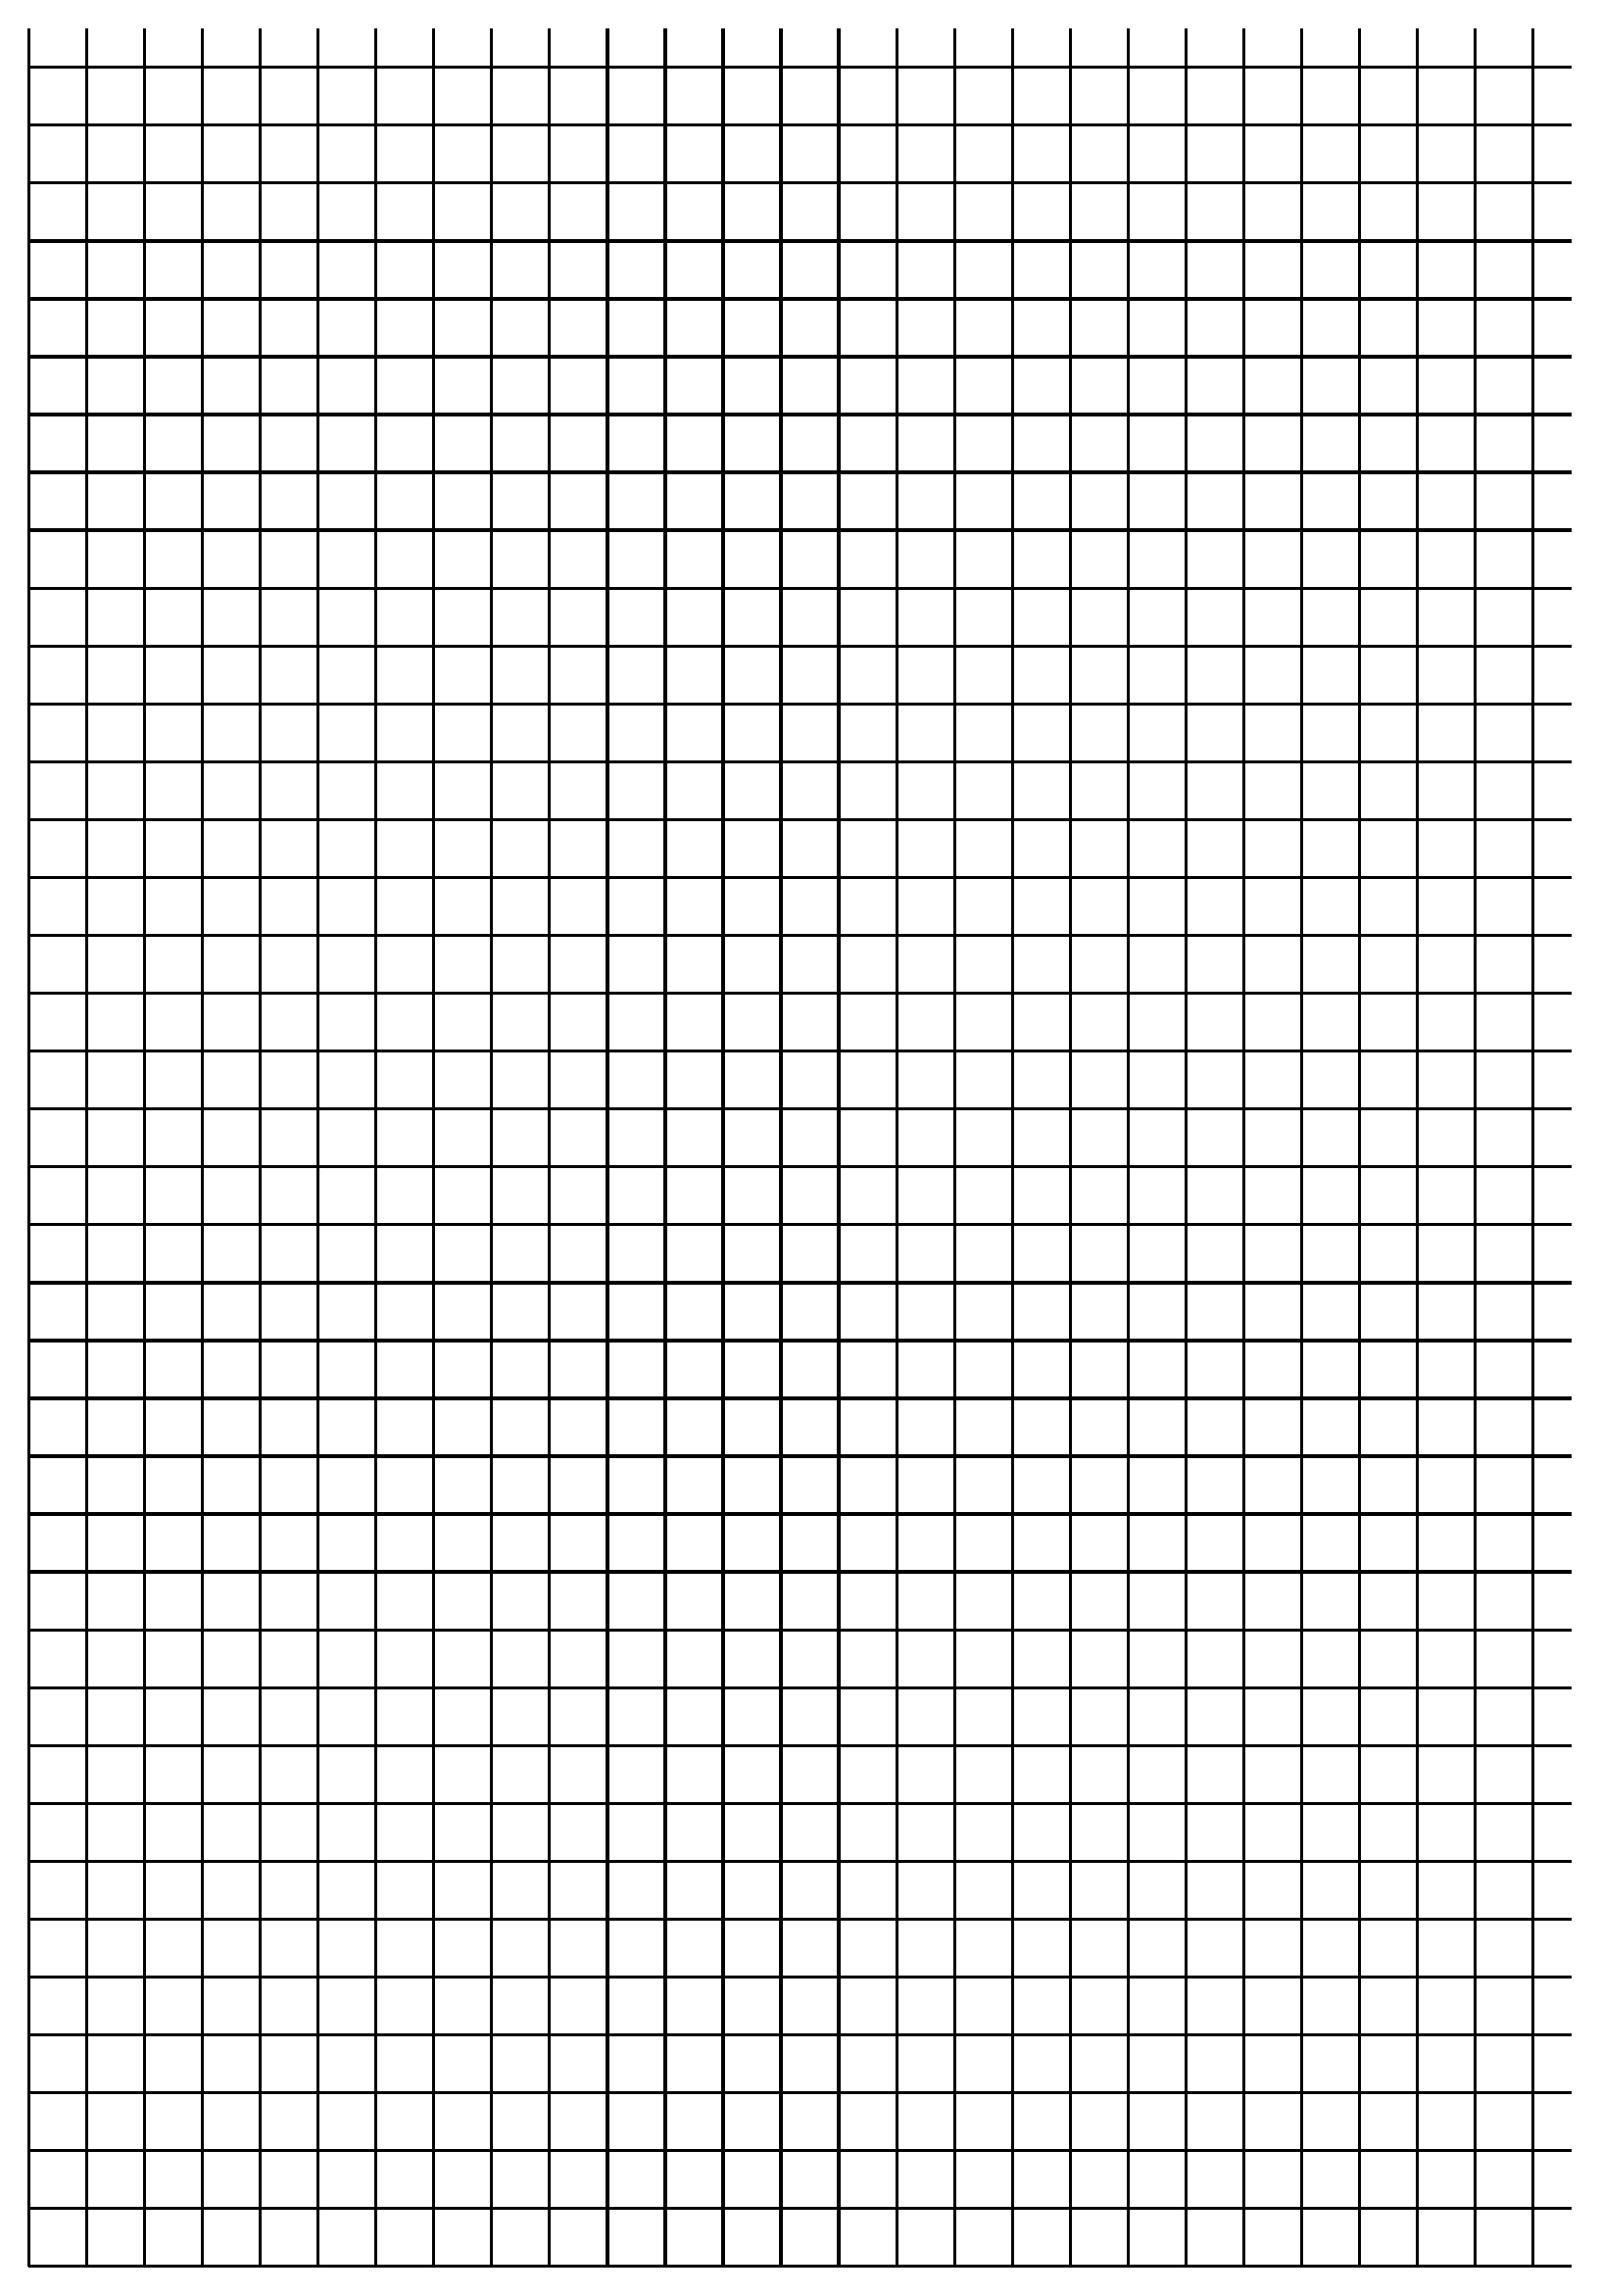
\begin{tikzpicture}
    \draw[step=0.75,very thick] (0,0) grid (20,29);
    % \foreach \x in {0,2,...,18} {
    %     \foreach \y in {0,2,...,22} {
    %         \pgfmathtruncatemacro{\shade}{mod(\x/2+\y/2,2)}
    %         \ifnum\shade=0
    %             \filldraw[black!70] (\x,\y) rectangle (\x+2,\y+2);
    %         \fi
    %     }
    % }
\end{tikzpicture}
\end{document}